\chapter{Block chain as infrastructure of semantic web}[paper6]



\section{Distributed ledgers and indexing}[p1431]
Distributed ledger based on blockchain do not have central control. Blockchains are organized into multiple blocks that initial block created manually and the other blocks are added by some consensus process between nodes.
Ethereum smart contract provides possibility of to control automatically what happen with cryptocurrency on the blockchain without involving the untrusted external sources. Ethereum smart  contracts has account which can normally store, update or making function with the input and output.
The concept\textit{accounts} are widely used in this study refer to agent such human and the concept \textit{balance} refers to cryptocurenccy in blockchains. \\ 
As already said, smart contracts are time-ordered where data are stored into blocks. therefore it requires the data to index. Indexing the smart contract, gives us capability to access the data, search, analysis services on the distributed ledger and expose them to outside the worlds for more of interactions.
There are different levels of indexing smart contracts: Basic level is the fundamental level for next step.It index basic entities such as account, blocks related to distributed level and data can be stored or retrieved here. In functional level, smart contracts contains alot of functional interfaces that depict the other functionality of platforms such as Ethereum. [p1431]
 There are not such comprehensive vocabularies to describe such concepts but some vocabularies are purposed in this case such as: 
\\
\textbf{FlexLedger}   
\textbf{BLONDiE and EthOn}  are formalisations of blockchain concepts
as ontologies, generic across Bitcoin and Ethereum blockchains and specifc to
Ethereum, respectively. It discuss initial approaches to Linked Data
indexing of blockchains, and the certication of Linked Data temporal streams
on blockchains, but both are very preliminary.[53]
  
 \section{Vocabularies}[p1431]
 \subsection{Why do we use ontology for Blockchain?}
 GEnerally, Blockchain is the destrubuted database that replicated over all nodes as s cloud computing arcitecture. These databases are distributed across noumerous organizations. That's why standard interpretation is needed that the data would be understandable by organizations. Interpretations are applicable via formal specification that enable verification and inference within software and applications executed on network. \\
 This is where ontology to play to ensure common interpretation of data of shared database among different intersperses. Blockchain modeling is the one form of modeling among enterprises.
 blockchain modeling used different type of ontology: informal ontology, semi ontology to facilitate search and enhance better understanding of business process for developing and applying on blockchain. Blockchain modeling based on formal ontology help the formal specification to verify the operation of blockchain. On the other word, blockchain modeling based on formal ontology can help the development of smart contract to execute on blockchain.\\
 Also, we can use ontology tocapture data within blockchain: From one hand, It facilitates the better understanding of blockchain concepts for human.On the other hand, enables interlinking with other link data to convey deductions and formal reasoning.[2]\\
 Vocabulary used within ontology increase the transparency of transaction in a way that by describing transaction in the context of linked data comfort the graphical represantation of location of such transaction. Thus , it increases also the capability of analysis by users.
   
 \begin{center}
 
 	
 	\begin{figure}[htb!]
 		
 		\begin{minipage}{0.55\linewidth}
 			\centering
 			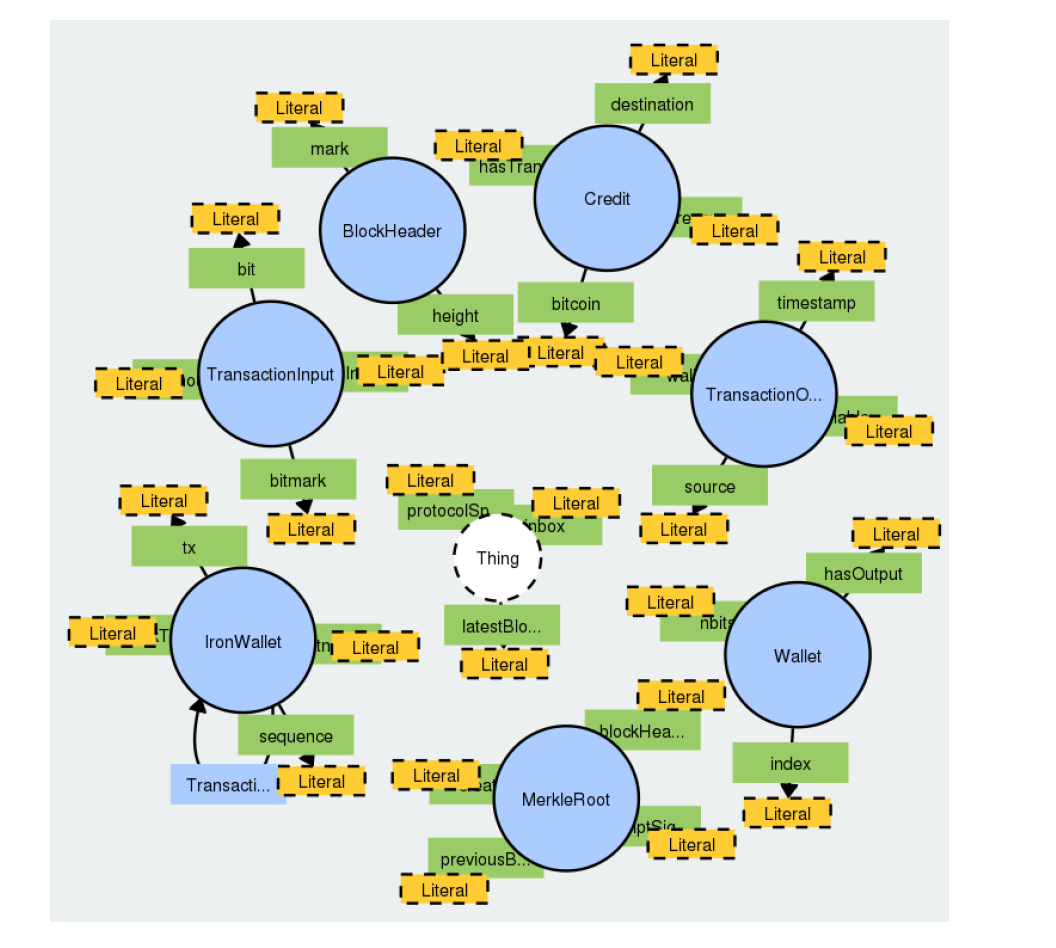
\includegraphics[width=1.65\textwidth]{images/chap02_diagram_ontology.png}
 		\end{minipage}
 		\caption[Illustration of Ontology diagram]{Illustration of Ontology diagram(2)}
 		
 		
 	\end{figure}
 	
 \end{center}
 
\subsection{Linked Data}
TODO
when information can represenr in linked data, querying about realted information can be easily discovered in linked data. It is based on 4 rules:

	\textbf{URIs}(Uniform Resource identifier) as names.\\ 
	\textbf{HTTP} to search for names.\\
	\textbf{(SPARQL, RDF)}  when a user search for something, provides related information.\\
	\textbf{Link} to other URLs to provide more information.\\


\subsection{Resource Discription Framework}
It is w3c specification that model information.
TODO
\subsection{SPARQL}
TODO
\subsection{Ontology and OWL}
TODO
Ontology Wen Language is made to represent knowledge bout things and the relations among them. OWL is computational logic-based language ,means the language modeled in OWL can operated in computer program like negation, intersection and so on. TODO

 \subsection{Vocabulary in Distributed Ledger}
 In ord is replecated over allnr to generate link data, it requires to use a standard ontology or vocabulary to explain the blockchain concepts. Interfaces between distributed ledgers and the Semantic Web are still on early stage in this. there are some systems that have such voicabularie includes: Flex Ledger, EthOn, BLONDiE[p1431].\\
 
 \textit{FlexLedger}: describes HTTP interfaces to blockchains, with a standard vocabulary and responses of these interfaces[p1431]. FLexLedger is a protocol for decentrelized ledger and interfaces which represent ledger creation, querying and data model using JSON-LD. However, Flex Ledger does not have explicit vocabulary about ontology nor  having concrete ontology for itself. 
 \\TODO It is also worth mentioning that the Flex Ledgermeta and the content data are stored together in the same graphwhereas the GraphChain blocks’ content is store outside the blockin a separate graph. For all the reasons stated above, GraphChaincannot be considered as an implementation of Flex Ledger.[p1171]\\
 \\
 \\
 \\
 \\
 
 \textit{EthOn} is an OWl ontology that describes blockchain concepts such as \textit{"blocks, accounts, message"}and relations such \textit{"has parent block"}.[40] TODO
 \begin{center}
 	\begin{figure}[htb!]
 		
 		\begin{minipage}{0.55\linewidth}
 			\centering
 			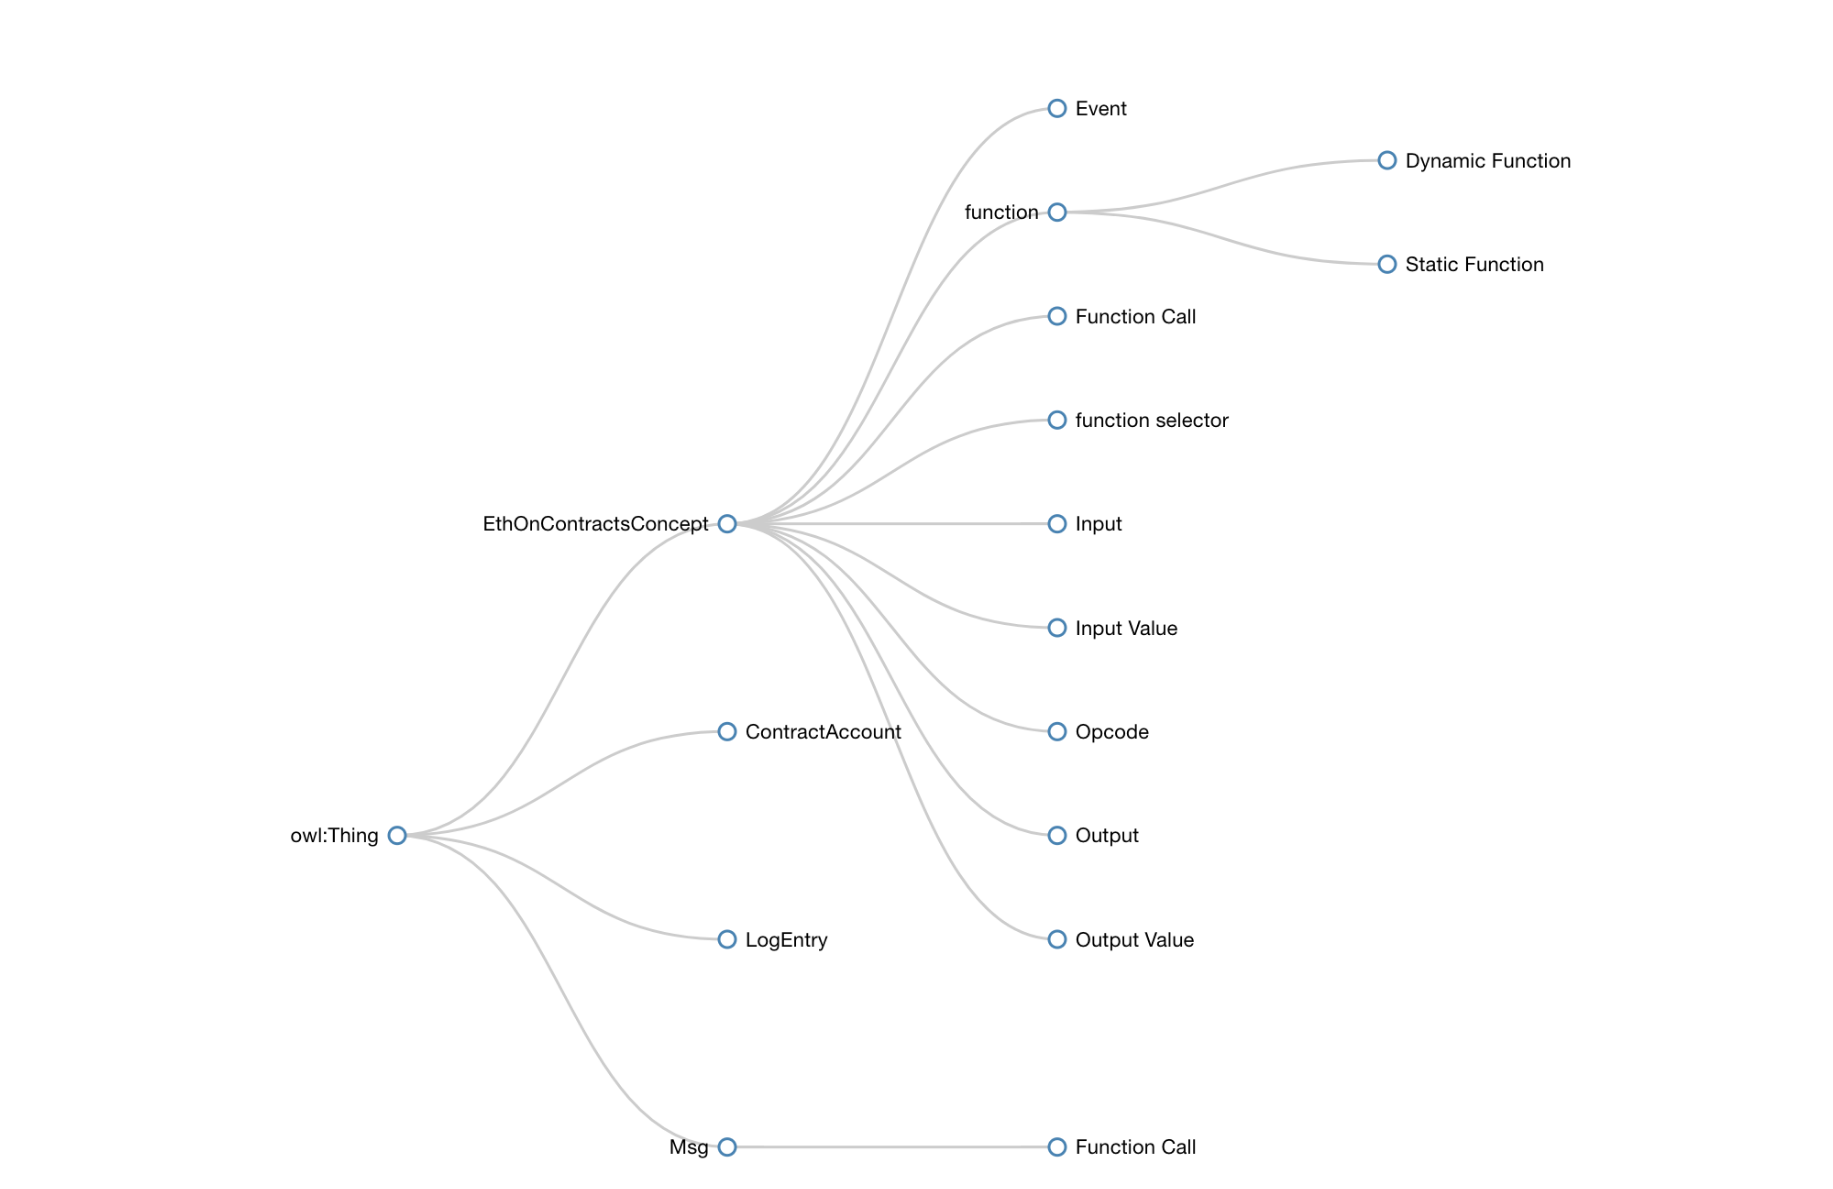
\includegraphics[width=1.85\textwidth]{images/chap01_EthOn.png}
 		\end{minipage}
 		\caption[EthOn classes]{EthOn Classes(negotitaion)}
 	
 	\end{figure}

 	\begin{figure}[htb!]
 		
 		\begin{minipage}{0.55\linewidth}
 			\centering
 			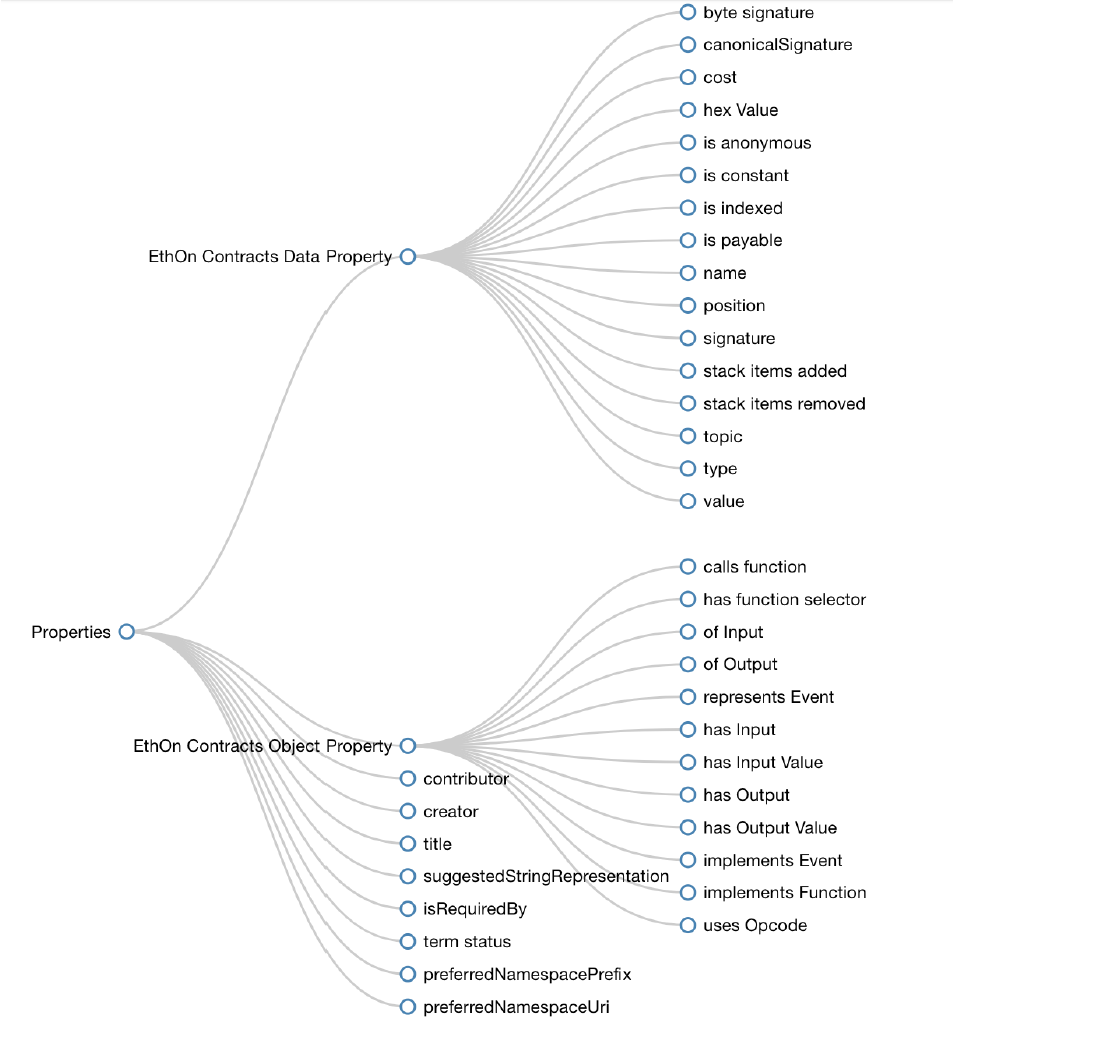
\includegraphics[width=1.65\textwidth]{images/chap02_EthOn_Properties.png}
 		\end{minipage}
 		\caption[EthOn Properties]{EthOn classes(negotition)}
 		
 		
 	\end{figure}
 	
 \end{center}

\textit{Blockchain Ontology with Dynamic Extensibility(BLONDiE)}
	
BLONDiE is another OWL ontology for describing the
Blockchain structure like EthOn. But is is more generic then EthOn. For example EthOn and BLONDiE bothe defined some terms such 'account', 'block', 'transaction' and some attributes such as 'transaction payload' or 'miner adddress'. BLONDiE defines some other concept for different Blockchain such as 'BitcoinBlockHeader' and 'EthereumBlockHeader' as sub classes of 'BlockHeader'. At the moment, BLONDiE supports two crypocurrencies like bitcoin and Ethereum where all link and relation between objects and attribute represent in RDF(Resource Description Framework).[p1431]
\begin{center}
	\begin{figure}[htb!]
		
		\begin{minipage}{0.55\linewidth}
			\centering
			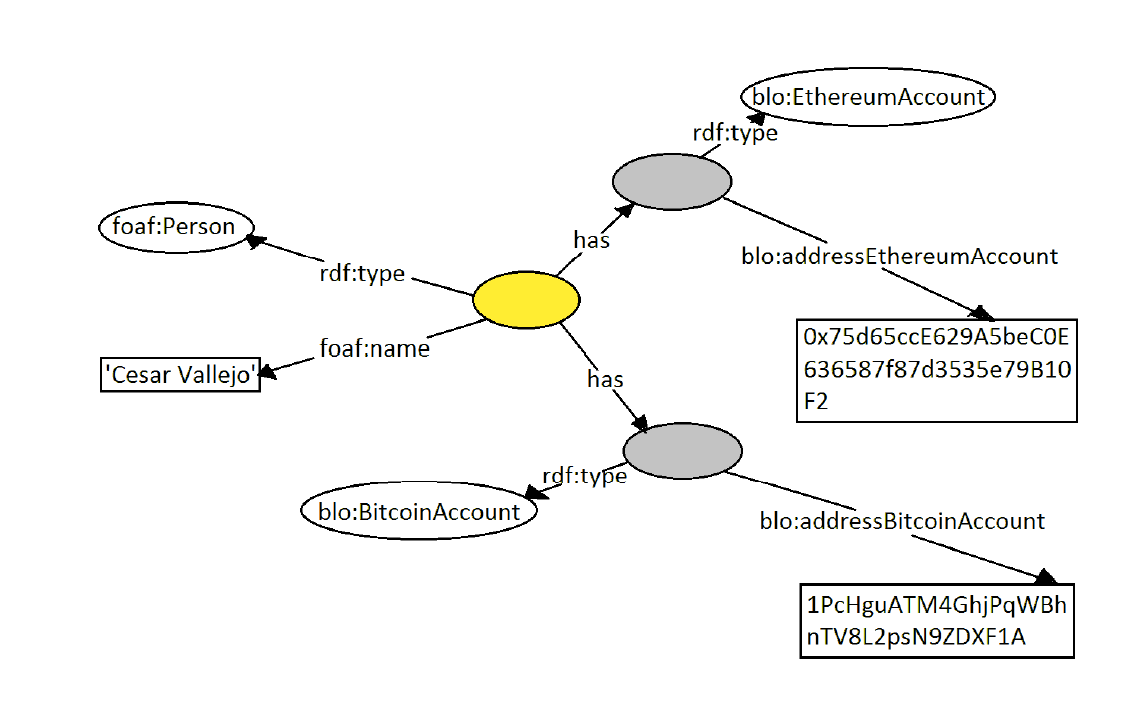
\includegraphics[width=1.95\textwidth]{images/chap02_BLONDiE.png}
		\end{minipage}
		\caption[BLONDiE]{BLONDiE usage example[45]}
		
		
	\end{figure}
	
\end{center}

\subsection{Linking Blockchain in BLONDiE[45]}TODO
On a general point of view, the Web is a huge global graph
of connected hypertext documents by hyperlinks. On a similar
way, there are some projects working in the idea of connecting
different Blockchains. Where the main goal is to create “the
Internet of Blockchains”. Since payments are different from
plane information, it can be copied and replicated, but money
must not be.
The interledger protocol (ILP)8 is for payments across
payment systems. ILP models the world of finance as a giant
global graph of ledgers connected by liquidity. The systems
providing this liquidity are called connectors and a key feature
of ILP is that these connectors do not need to be trusted,
meaning anyone can create one [21].
Currently, centralized exchange platforms are used to exchange
one Blockchain-based currency for another. Cosmos9
is a network of Blockchains, organized on hubs and zones.
Zones plugged into a central hub and each zone maintain
its each governance. Allowing the decentralized exchange of
tokens from one Blockchain to another.
Polkadot10 is a new network that aims to provide interoperability
between private and public Blockchains. Allowing
extensibility and scalability. It defines a heterogeneous
multi-chain, provided to an absolute minimum of security
and transport. Scalability is addressed through a divide-andconquer
approach. The heterogeneous nature of this architecture
enables many highly divergent types of consensus systems
interoperating in a trustless, fully decentralized “federation”,
enabling open and closed networks to have trust-free access
to each other [23].
Two more similar projects are Blocknet11 and Supernet12.
All these projects show evident need of semantic empowerment.
The same need that the web still has to really jump from
an only “Syntactic Web” (Web of documents) to a “Semantic
Web” (Web of data). While how and where to locate and
enable semantic data is not completely clear, it is obvious
that Semantic Web fits as a prominent set of technologies to
be used here. In Figure 4, we present datasets that have been
published in Linked Data format by contributors to the Linking
Open Data community project and other individuals and
organizations. In a similar way, Blockchains-based systems
and its corresponding datasets can be published and linked.

\begin{center}
	\begin{figure}[htb!]
		
		\begin{minipage}{0.55\linewidth}
			\centering
			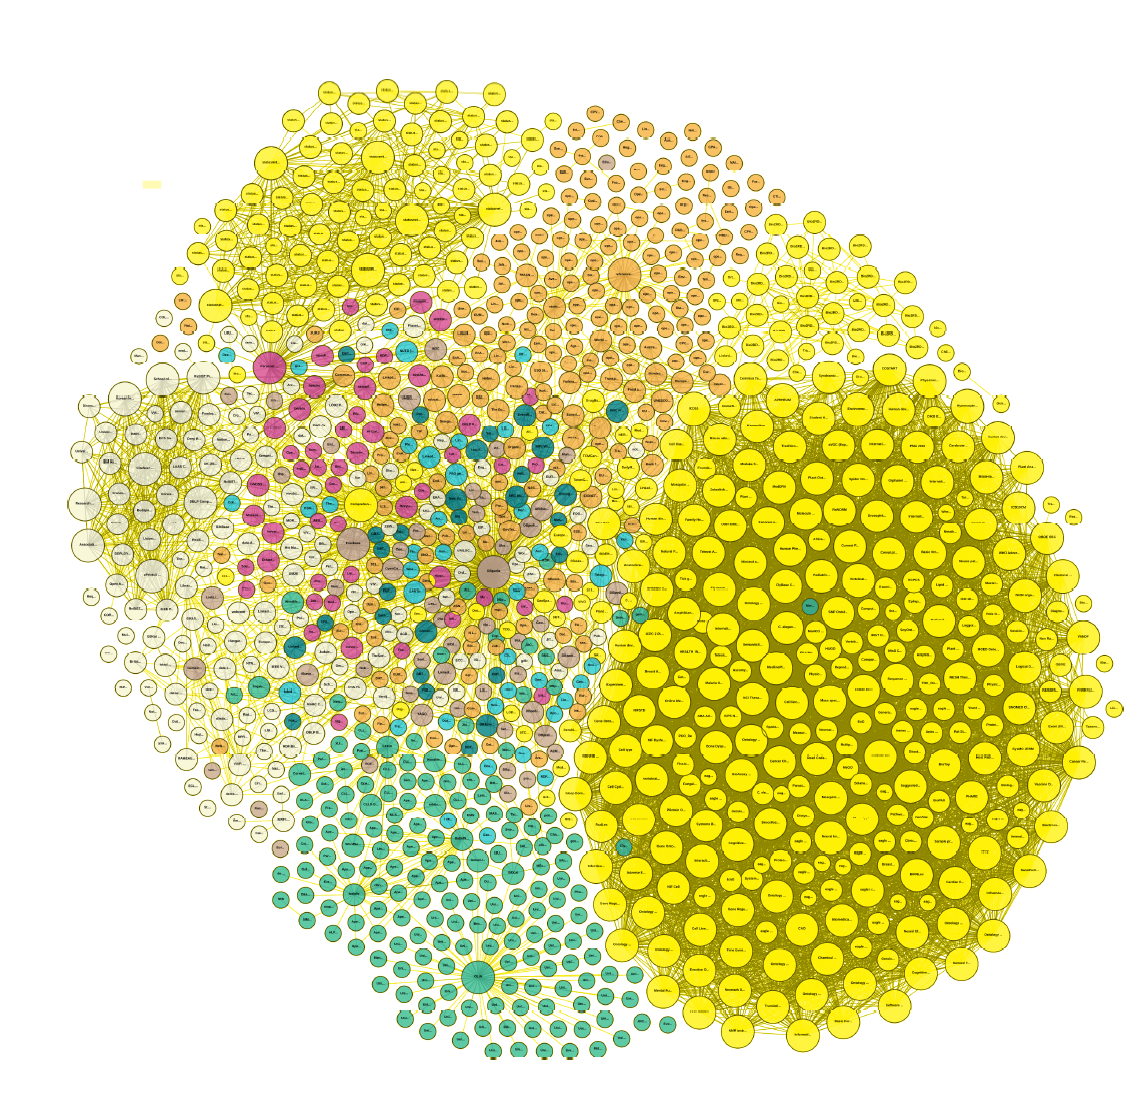
\includegraphics[width=1.95\textwidth]{images/chap02_LinkData.png}
		\end{minipage}
		\caption[Linked data diagram]{Linked data Diagram[45]}
		
		
	\end{figure}
	
\end{center}

\subsection{Ontology-based smart contract in BLONDiE[45]}
Data models are used on Ontology-Based Object-Oriented
Enterprise Modelling [24]. In a similar manner, Kim and
Laskowski [25] propose that ontologies can contribute to
Blockchain design. Their approach can aid in the development
of Smart Contracts that execute on the Blockchain.
They come up with a proof-of-concept using Ethereum
and TOVE Traceability Ontology. This interesting idea can
be replicated for other ontologies too. Better data standards,
business practices and processes for developing and operating
Blockchain are achieved. It also aids in the formal specification
for automated inference and verification in the operation of a
Blockchain.[45] TODO

\subsection{Storage and RDF}
The main goal of data over web is to make data machine readable format on web. It causes to interpret data in suitable formats to be useful in a way that be human readable too. \\
JSON-RPC is remote procedure call protocol in JSON. his protocol allows to send data to server without needing to response. 
Ethereum blockchian which has properties such as pay 
fee with Gas, there are different was of storing data in RDF triple
Most wallet in Ethereum in in JSON format that is seasily convertble to RDF and fornt-end is made up with HTML  technology that we can use it to embed data on website interface as Micro data, JSON-LD. The main focus of research is the storage of data on blockahain itself.There exist limitation of storage in Ethereum blockchain and to fees. that's why, it is suitable to use compact RDF serialization.[45] There are some methods to store data on Ethereum  blockchain that are summarized in table bellow:
\begin{center}
	\begin{figure}[htb!]
		
		\begin{minipage}{0.55\linewidth}
			\centering
			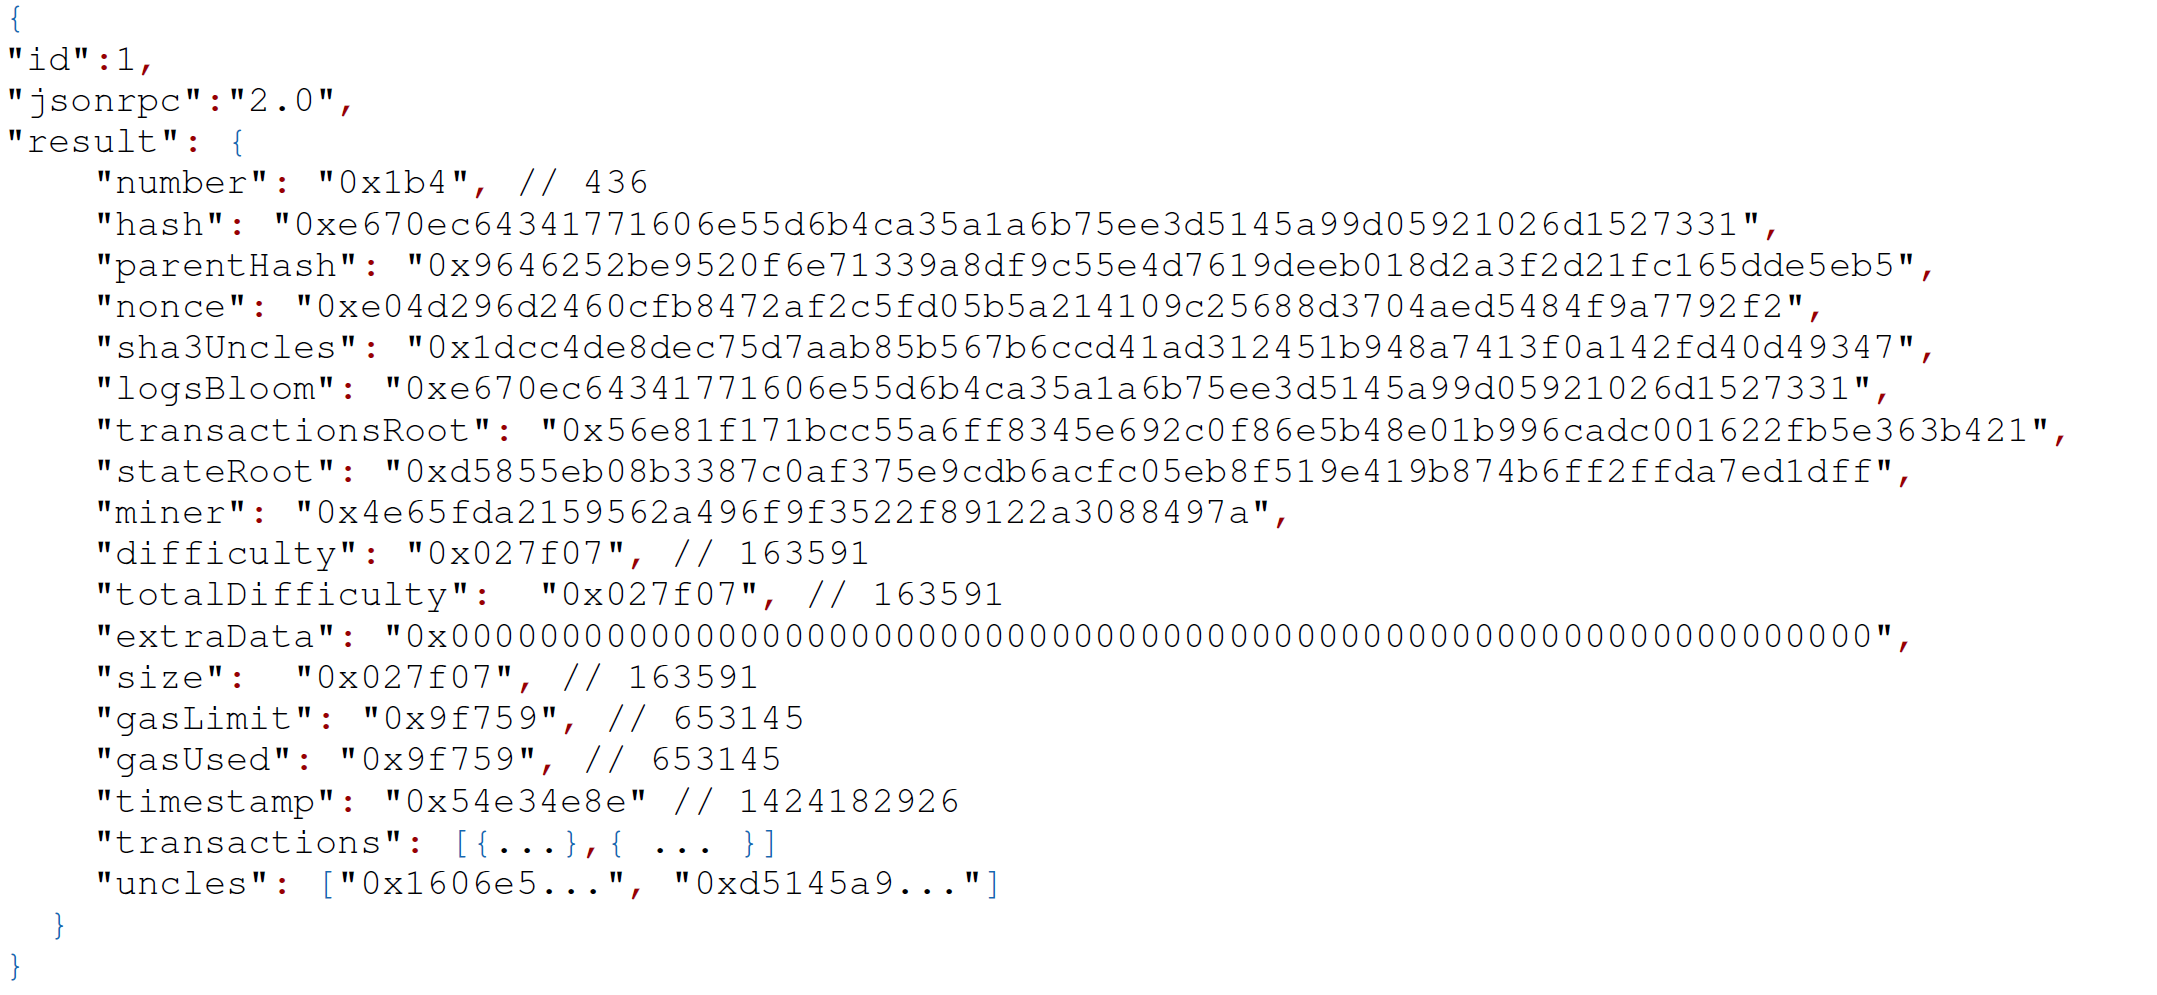
\includegraphics[width=1.95\textwidth]{images/chap02_Eth_str.png}
		\end{minipage}
		\caption[Ethreuem structure]{Ethereum structure}
		
	\end{figure}
	
\end{center}
\begin{center}
	\begin{figure}[htb!]
		
		\begin{minipage}{0.55\linewidth}
			\centering
			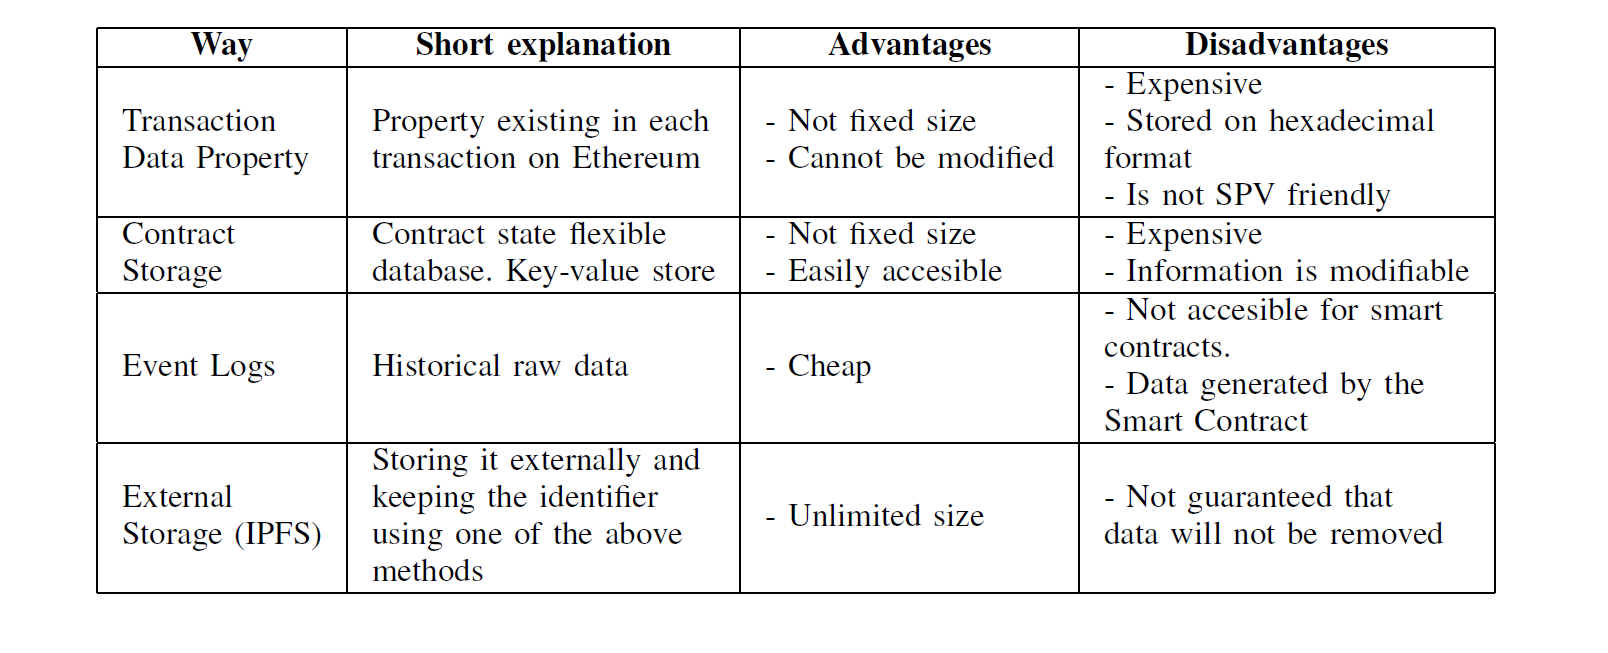
\includegraphics[width=1.95\textwidth]{images/chap02_Eth_Table.png}
		\end{minipage}
		\caption[Storage of RDF data on Ethreuem summery]{Storage of RDF data on Ethreuem summery}
		
	\end{figure}
	
\end{center}



\subsection{Semantic Blockchain}
	
By increasing of the usage of blockchain technology recently, the need for semantic reasoning on distributed ledger is on crease as well. The blockchain is the best platform to utilize semantic web principle inthis technology and add new trusted property to dataset. that makes new dataset so thruthworthy. 
Using semantic web technology on blockchain in novel idea and the way of how apply this technology in blockchain and smart contract is also as controversial issue.\\
There are some \textbf{definition of semantic blockchain:}\\ 
\textit{Semantic blockchain is the representation of stored data on distributed ledger using linked data. }\\
\textit{Semtcic blockchian is the applying semantic web standard on blokchain that these standards is based on RDF.}

\subsection{semantify Blockchain process}
Semantic blockchain or semantic distributed ledger has effect on industrial world and subsequently , the result lead to start developing new application and framework to combine two worlds:
thee are some way to semantify blockchain:
\textbf{-}Mapping the basic blockchain to RDF making usege of vocalbularie, ontology and so on.
\textbf{-} Storage of data in blockchain is expensive, The only wey is to store the hashing point to data set in blockchain and then share RDF on blockchain.
\textbf{-} Create semantic blockchain that internal data exchange protocol is based on RDF.

TODO
SemBlocRouter [45]
\subsection{Semantic Ontology Mapping}[p1341]
To generate RDF, ot is need to ap the basic blockchain  etities to relevant semantic web terms, concepts and ontology. In order ot make query more efficent BLONDiE used some ways such as:\\  
Firstly, records realting to block and transactions both, have been completed with attribute for hashing to provide direct mapping between contents of index and address of entities on blockchain, Secondly, transaction with link to blocks or smart contract and input to smart contract.\\
Blockchain stores just binary form of each contract with metadata.   
it requires to have the relevant Application Binary Interface (ABI) specification in JSON form to interact with such contract. This specification is created when the smart contract is compiled and stored in blockchain. Indexing of smart contract on blockchain is in binary form. IN order to interact with contract Application Binary(ABI) Interface specification is needed. This specification is in the form of JSON and is created when smart contract is compiled and stored in blockchain. The ABI determines all functions of contracts and description about input, output parameter for each contract.
 
\begin{center}
	\begin{figure}[htb!]
		
		\begin{minipage}{0.55\linewidth}
			\centering
			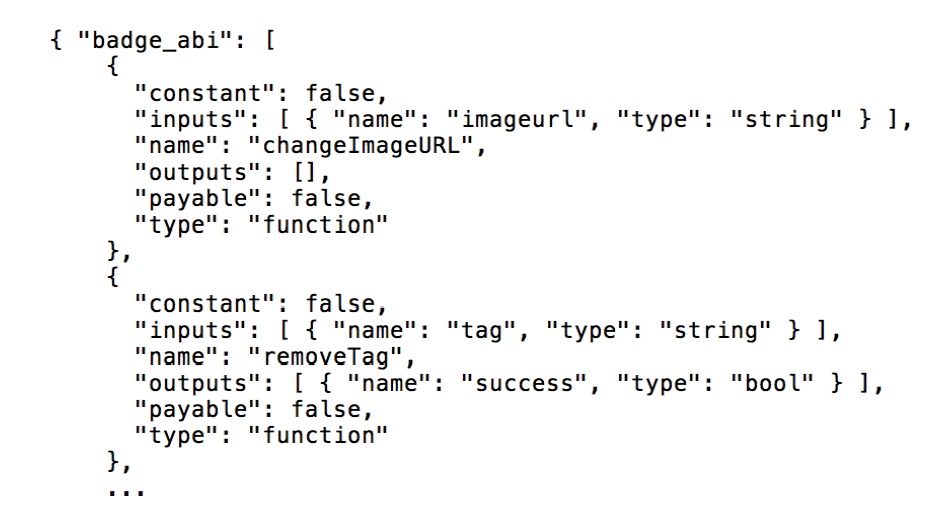
\includegraphics[width=1.95\textwidth]{images/chap02_SmartContract_ABI.png}
		\end{minipage}
		\caption[Smart contract of ABI]{Smart  contract of ABI}
		
	\end{figure}
	
\end{center}
By the use of ABI, it generate RDF to index smart contract.
Author()model smart contract as follow:\\
- A contract as \textit{msm:Service}\\
- A function as \textit{msm:operation} with (\textit{msm:hasInput} or \textit{hasOutPut}) related to suitable \textit{msm:MessageContent}\\
- A msm:Service records contains the blockchain address as an attribute to keep the index into blockchain.
 

\subsection{Vocabulary in Smart Contracts}[p1341]
As already menthiond, EthOn and BLONDiE are both similar concept that can be used for smart contract. as, smrt contract is the executable  software, so the semantic and vocabularies that are applicable for other software too.\\
There are many works on semantic annotation of web (see [AnnaFensl]) and HTTP APIs which may enable us to annotate smart contract as well. However, the caontracts are not Web API and implementation ma differ but the main concept does not differ.  On the other word, the vocabularies used to annotate web services, are usable to annotate smart contract too. It is seems that the Combination of distributed ledger with smart contract and web service due to profitability  become common.
\\ Here, Author(TODO negotation author) used Minimal Service Model(MSM) with Ethereum Ontology(EthOn) to describe some concept of smart contract like Gas and son on that make us enable to answer queries such as 'finding a smart contract with the minimal gas payment'.

\subsection{Minimal Service Model}[negostation]
The MSM defines a service that has Operations. Operations   have input, output and fault MessageContent that may include mandatory or optional MessageParts. MessagePart provides support for finer-grained input/output discovery, as available in SAWSDL, OWL-S and WSMO

 \begin{center}
	\begin{figure}[htb!]
		
		\begin{minipage}{0.55\linewidth}
			\centering
			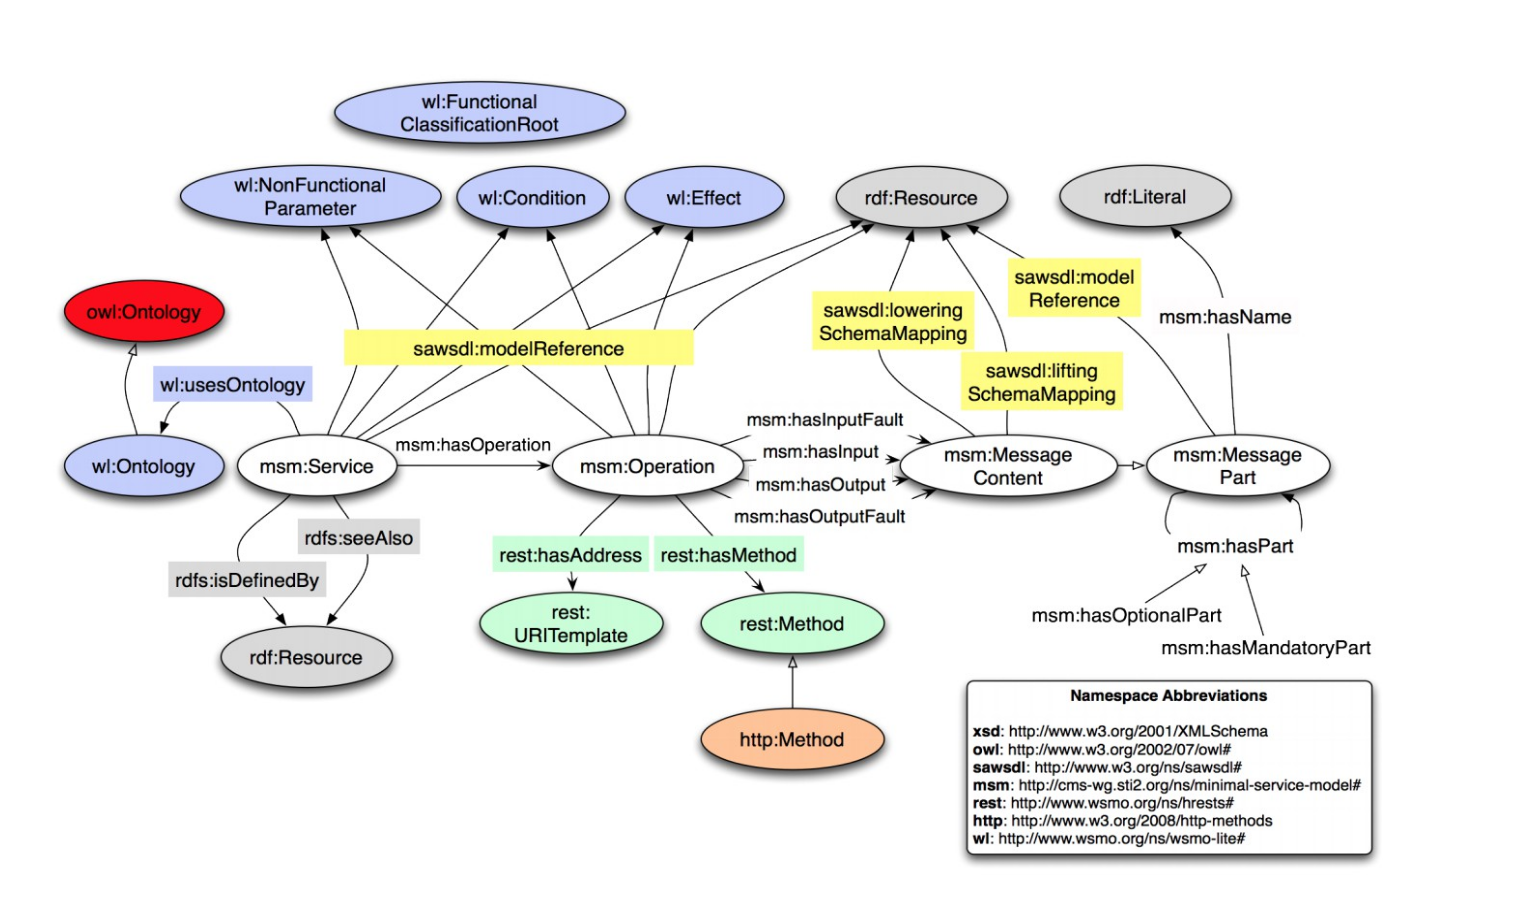
\includegraphics[width=1.95\textwidth]{images/chap02_MSM.png}
		\end{minipage}
		\caption[Illustration of Minimal Service ModelOntology]{Illustration of Minimal Service Model Ontology nrgotation}
		
	\end{figure}
	
\end{center}
We present one example that Author() used to clarify more the meaning of MSM in blockchain: Inthis example, educational data is used to store in blockchain using Ethereum \textit{web3} library.\\
Author()considered that every block add to blockchain and retrieve trascation within block. If transaction contains smart contract.Then it retreive contract address using Ethereum API. Then, it sves the smart contract address, Application Binary Interface(ABI) as triple in RDF. ABI describes the name of smart contract and way of calling them. Auther, then saved each method in ABI as an RDF triple based on MSM ontology as follow:

\begin{center}

\begin{tabular} { c | c }
	 
   \textbf{Smart Contract Methods} & \textbf{MSM}\\
	\hline
	Smart Contract ABI & msm:service\\
	\hline
	Function   & msm:opreation\\
    \hline
	 Input   & msm:messagecontent\\ 
	 \hline
	 Output   & msm:messagecontent\\ 
	 \hline
	 Gas   & msm:gas(from EthOn Contract DataProperty 'cost')
	
\end{tabular}

\end{center}
   TODO MY example  		
	
\subsection{Implementation of BLONDiE}[p1341]
			
 \section{Link Data TODO}[45]
 According to Tim Berners-Lee, Linked Data is “the Semantic
 Web done right, and the Web done right”. When information
 is presented as Linked Data, other related information can
 be easily discovered and new information can be easily linked
 to it. It is based on these 4 rules [8]:
 i) Use URIs (Uniform Resource Identifiers) as names for
 things.
 ii) Use HTTP URIs so that people can look up those names.
 iii) When someone looks up a URI, provide useful information,
 using the standards. (RDF, SPARQL)
 iv) Include links to other URIs. so that they can discover
 more things.
 \subsection{RDF[45]TODO}
 The Resource Description Framework (RDF) is a family
 of W3C specifications, “it is a foundation for processing
 metadata” [9]. On web resources, RDF is used as the standard
 way to describe and model information. Three object types
 conform the basic model [9]:
 i) Resources. The things that where RDF expressions are
 used to describe them.
 ii) Properties. The specific description of a resource, it can
 be an attribute or a relation.
 iii) Statements. The conjunction of a resource, a named
 property and the value of that property. These three
 elements form the RDF statement of a specific resource.
 They are expressed in the form of subject, predicate,
 object and commonly called “triples”. Triples create a
 basic graph structure of data.
 Definition 4. RDF triple. An RDF triple t is defined as a
 triple t = (s,p,o) where s 2 U [B is called the subject, p 2 U
 is called the predicate and o 2 U [B[L is called the object.
 where: U (Set of all URIs), L (Set of all literals) and B (Set
 of all blank nodes) [10].
 
 \subsection{SPARQL[45]TODO}
 SPARQL (recursive acronym for SPARQL Protocol and
 RDF Query Language) is a W3C recommended semantic
 query language for datasets, it is made for retrieving and
 handling data stored in RDF format. Thus, the queries are
 working over a graph structure defined by the RDF data, where
 the result will also be a graph or a subset of it.
 \subsection{OWL[45] TODO}
 An ontology is a set of explicit formal specifications of the
 terms (classes or concepts) in a domain and relations (properties
 or roles) between them [11]. When a set of individuals
 (instances) is available, it is known as a knowledge base. Ontologies
 define a common vocabulary for researchers that want
 to share information in a domain and they include machinereadable
 definitions of basic concepts and its relations [12].
 Web Ontology Language (OWL) is a language made to
 represent complex and rich knowledge about things, sets of
 things and existing relations between them. OWL documents
 or OWL ontologies are usually published on the WWW and
 make reference or be referred from others OWL documents.
 OWL is a computational logic-based language meaning that
 knowledge modeled in it can be exploited by computer programs,
 e.g. to make implicit knowledge explicit available [13].
 It has a rich set of operations like union, negation, intersection,
 etc. Its logical model allows the use of reasoners that are
 checkers of consistency between ontology elements.
 \subsection{WEB3 [45]}
 
 \section{Retrieve Information form semantic blockchain}[paper6]
 Reasoning and knowledge representation in semantic web are based on Description Logic(DL). Description logic has some elements such: classes and properties , link between different object and etc. Ontology is the study about the objects and relations between these objects or entities.
 An individiusl axiom also known as \textit{fact} forms a assertion box. Asssertion box and ontology together create knowledge base.\\
 Our work extens, in the keepong with the retrieving thge most relevent resources for given query by requester, where both query and resourcse are matched called as semantic matchmaking. This proccess leads to two approach \textit{full macth}, \textit{no match}.TODO  
 First, Resources and query may not matched. So one contradiction determines the location of infliction with resources. if one retracts, query TODO
 Second, if resources and query matches. But resources are not full match in ......
 
 Logic based matrix 
 \subsection{Semantic Blockchain Architetuer} 
 This method purposed framework based on semantic discovery layer built up on basic blockchain. It is striking to see the main features of such a blockchain as follow:
 
  \begin{center}
 	\begin{figure}[htb!]
 		
 		\begin{minipage}{0.55\linewidth}
 			\centering
 			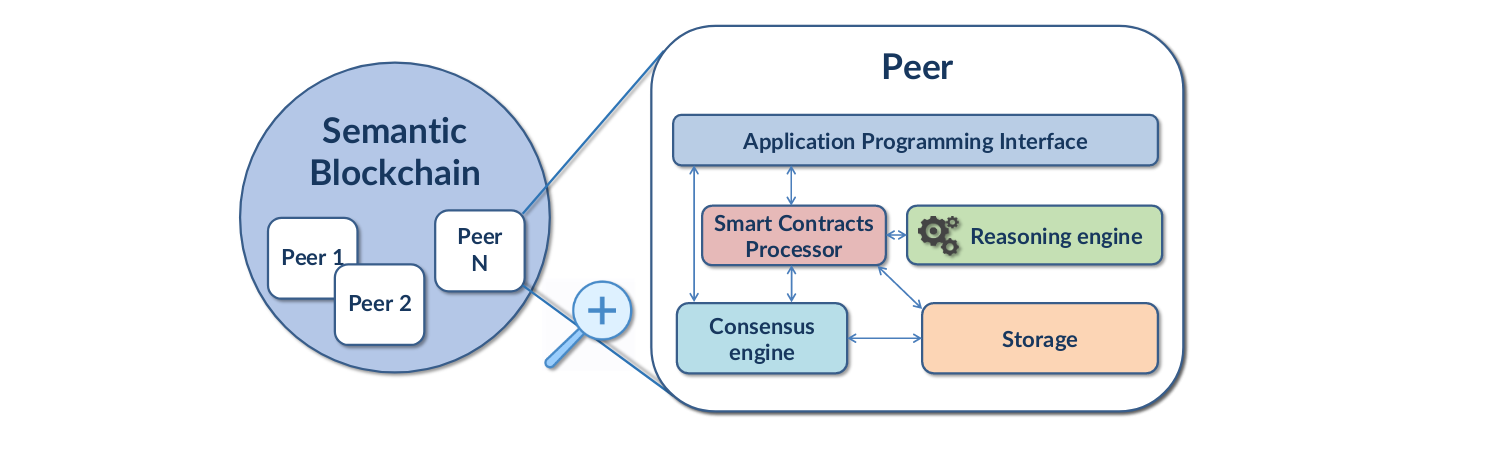
\includegraphics[width=1.95\textwidth]{images/chap02_PeerBlockchain.png}
 		\end{minipage}
 		\caption[Framework Arciteture]{Framework Arciteture (semantic web of thing)}
 		
 	\end{figure}
 	
 \end{center}
 
 
  \textbf{Peer} agent is identifed bx public key and its acounts. Each agent is able to enforce semantic discoveryto transfer asset between annotations that are stored in blockchain. And each peer is the integrated of matchmaking and reasoning engine for semantic discovery.
 
 \textbf{Asset} represents the resources and service instances based on domain ontology.\\
 \textbf{Smart Contracts} are the integration of matchmaking and reasoning engine.\\
 \textbf{Consensus Engine} allows to validate transaction in blockchain.\\
 \textbf{Storage} built up  \textit{markle tree} out of transactions including semantic ones to efficient detection of erroneous change in transaction.
 
 \subsection{Semantic in Consensus Protocol}[paper6]

 In semantic blockchain, EthOn or BLONDiE concepts and vocabulary to facilitate integrity and develop resource discovery. EthOn concept used W3CRDF schema and web ontology language to describe blockchain contract concepts. By the use of This concepts, it is possible to compare request with different recourse with respect ot semantic annotation of shared domain ontology. 
 Smart contract semantic is represented by service layer that gives correct description of discovery outcome. Thus, it raise the trust of discovery process for users. In semantic blockchain, Author() used domain ontology to maps to EthOn contract. These concepts used for OWL-s ontology, indexing and invoking smart contract on Blockchain via URIs.[semdec] 
 Semantic blockchain also preform operations such as: registration, discovery, selection and execution that are implemented as smart contract. 
  Author here focused on semantic mismatching as a significant feature of semantic blockchain  with respect to basic blockchain.  This allows to compute the semantic distance between resources and queries with the same ontology.
 The logic-base matrix enforce the semantic ranking liat of element of the query. \\
 
 
 
 \textbf{A:Resource Registration:}
   As already mentioned, Smart contract desined using OWL specification. It used concepts and entity defined as class in OWl language and relationship between entitites defined as object properties with regard to ontology. In order to construct smart contract semantic , requires framework to design such contracts.\\
   Multiple resources stored on blockchain and Each domain is related to a different ontology that provide vocabularies for annotating resources. Resources also are categorized by attributes such as: URI of reference ontology to retrieve the resource, semantic annotation in OWL that describe resources, resource price.
   In order to register resource on blockchain, 
   a user is required to register an account with public address and related private key to call the smart contract as parameter. 
   In ontology, a user describes as class corresponding to an account along with other attributes such as address, private key and other details. \\
   To acheive ths, A new ontology called \textit{EthereumContractConcepts} is implemented containing \textit{EthereumContract} data prperty. A \textit{ContratcAccount}
consist of lisencenumber, date, smart contract owner and state.
 After all, smart contract is developed with vocabulary  as domain-based-ontology. [semdec]  
 
  
 \begin{center}
 	\begin{figure}[htb!]
 		
 		\begin{minipage}{0.55\linewidth}
 			\centering
 			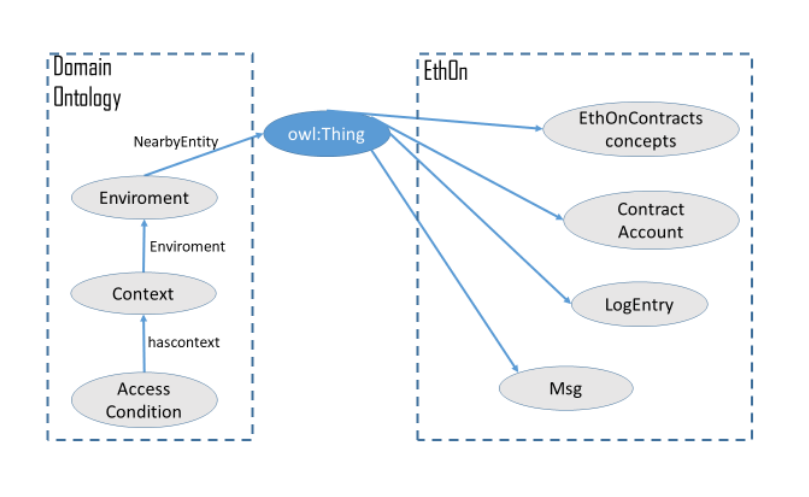
\includegraphics[width=1.95\textwidth]{images/chap02_Domain_EthOn.png}
 		\end{minipage}
 		\caption[Domain ONtology]{Domain ontology semdec}
 		
 	\end{figure}
 	
 \end{center} 
  
 \textbf{B: Smart Contract}
 Author used the EthOn and OWl concepts build semantic web service for smart contract. Autho() used OWL-S ontology that makes functionalities such discover, invoke and monitor by providing some additional vocabulary along with smart contract concepts facilitate query to finding smart contract. The OWL-S ontology provides three type of description about service as follow in figure():\\
 
 
  \begin{center}
 	\begin{figure}[htb!]
 		
 		\begin{minipage}{0.55\linewidth}
 			\centering
 			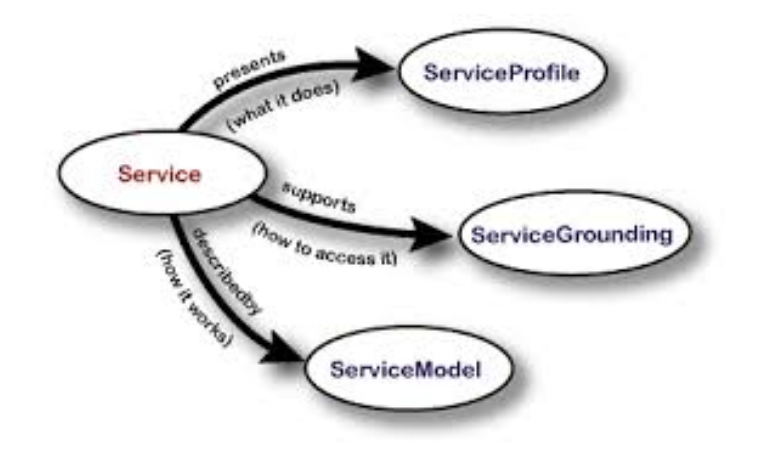
\includegraphics[width=1.55\textwidth]{images/chap02_SmartContract.png}
 		\end{minipage}
 		\caption[Service-based smart contract]{Service-based smart contract}
 		
 	\end{figure}
 	
 \end{center}
By the use of EthOn concepts, we can monitor the added block to blockchain. When a transaction has a smrt contract, ir is retreived the store contract address via API, then the address of smart contract and Application Binary Interface(ABI) as a triple in RDF store. ABI consist of the smart contract method and way of calling it. Methods are stored in ABI as an RDF triple with regard to OWL-S ontology. Table bellow show the OWL-s vocabulary to describe the smart contract[semdec].
\begin{center}
	\begin{figure}[htb!]
		
		\begin{minipage}{0.55\linewidth}
			\centering
			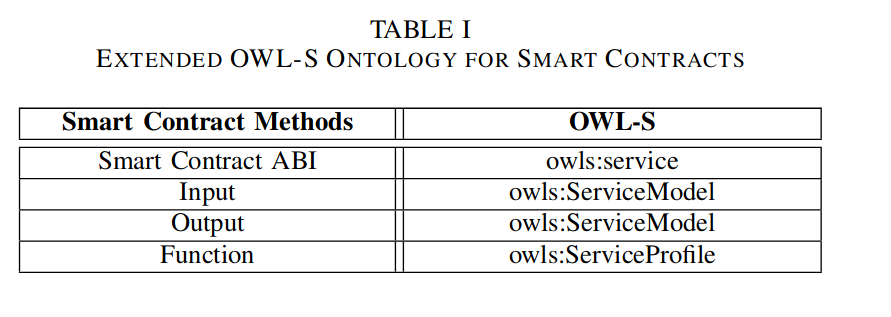
\includegraphics[width=1.95\textwidth]{images/chap02_OWL.png}
		\end{minipage}
		\caption[OWLS ]{OWLS ontology for smart contract} 
		
	\end{figure}
	
\end{center}
 \textbf{Semantic  Discovery of Semantic Smart Contract: }
 In order to search for a smart contract or an item, The requester send the request to $n$ nodes randomly specifying:\\
 - URI of domain ontology to determine resource and vocabulary of both resource and request which to be retrieved.\\
 - Semantic annotation of smart contract in OWL language. \\
 - Maximum price $p_max$ that requester pays.\\
 - Minimum semantic $s_min$ threshold in $[0,1]$ interval, 1 is related to full match and 0 is the mismatch. 
 - maximum result $r_max$ is to be returned.
 - Address of requester. \\ 
 Author() here used the $gossip$ approach to propagate the request. The nodes which received the request preform 2 operations at the same time: First, preform semantic matchmaking of own resource with the request and provides a list of max result $r_max$ satisfying both semantic relavance score $s_min$ and cost $p_i <= p_{max}$, is returned.\\
 Second, send the request to other $n$ nodes randomly, the other nodes preform at the same way until reach the $m$ thresholds. the request continue until reach the $\sum_{i=1}^{m} n^i$ with $n$ and $n$ parameters. Then do not forward the request and preform match making locally.\\
 Afterwards, the nods send back the result to main requester at the specified address[semdec].\\ 
 \subsection{Resource Selection:} After receiving all results, requester selects the best resource and smart contract, sending message to resource owner and contextually payment.the receiver responses with the proper resource representation relied on meaning of uri[4].
 The resource discovery and retrieval interaction is shown in Figure() and Each associated transaction is recorded on the blockchain[4].

 
 \begin{center}
 	\begin{figure}[htb!]
 		
 		\begin{minipage}{0.55\linewidth}
 			\centering
 			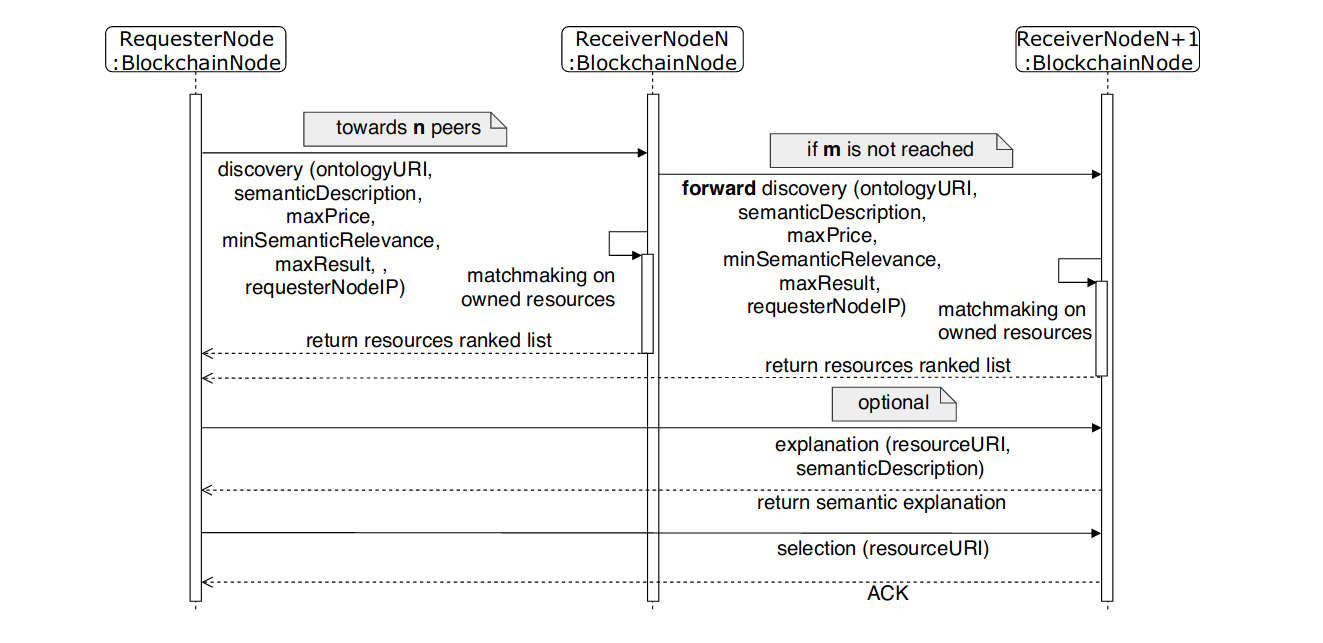
\includegraphics[width=1.95\textwidth]{images/chap01_SemanticBlockChain.png}
 		\end{minipage}
 		\caption[Resourse Discovery]{Resourse Discovery (4)}
 		
 	\end{figure}
 	
 \end{center}

\subsection{Indexng of Smart Contract}
As already mentioned, distributed ledger, does not have central registry due to their structure. Contract in this distributed ledger is not directly queried.
and blockchain is the time-ordered structure where data exist on multiple blocks.
In such distributed structure, developing the indexing process for smart contract is necessary. Indexing system provides a bility to analysis and search service on blockchain  and displays the outside.
There are differnet level of indexing such as low level to index basic entities such as account, transaction, block and top level for more functional operations is indexed.

\subsection{EthOn}
Is an ontology that describe blockchain concepts such transaction , account, block using w3RDF
 schema and ontology web language OWL to describe the relation these objects on blockchain.
In order to model data and be understandable for resource, EthOn and some semantic such as "hasParentBlock".
EthOn in at infancy and should develop more to have smart contract concept, functions, events, input and output and etc.
EthOn accepts consider just some relation between smart contract and Ethereum framework. There are multiple tools and language that can annotate smart contract. In this study Author() used OWL-S ontology due to some significant feature such as felxibility, widly discription of servic e and non- restriction ....
The main goal is to develop to support the smart contract too with respect to semantic web service context.
For reaching to this aim, web Araph chain is PI and smart contract can be represent as a executable function in distributed environment. Semantic web describes message, service and entities in machine readable format that can support logical reasoning based on semantic web service description. It helps mapping between different ontologies which faiciliate the concepts transformation among ontologies[semdec]. 

  
 \begin{center}
	\begin{figure}[htb!]
		
		\begin{minipage}{0.55\linewidth}
			\centering
			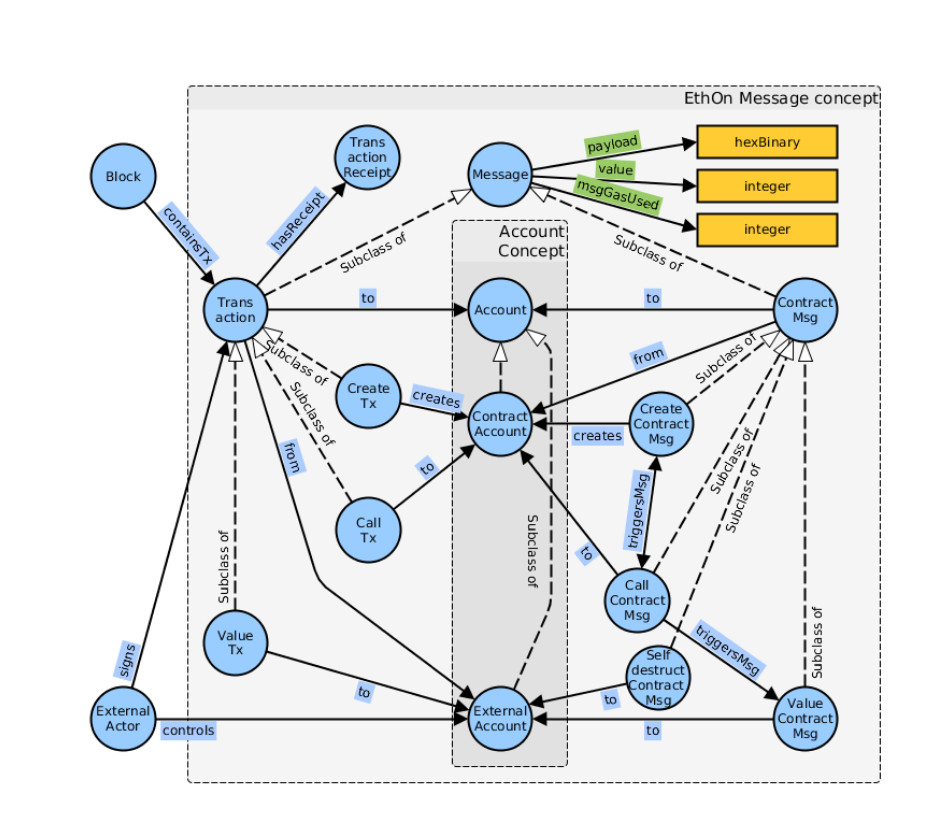
\includegraphics[width=1.65\textwidth]{images/chap02_EthOn.jpg}
		\end{minipage}
		\caption[EthOn message concept]{EthOn message concept}
		
	\end{figure}
	
\end{center}
\subsection{Smenatic Smart Contract}

 \section{Web 3.0}
 
 
 
 
 \begin{center}
 	\begin{figure}[htb!]
 		
 		\begin{minipage}{0.55\linewidth}
 			\centering
 			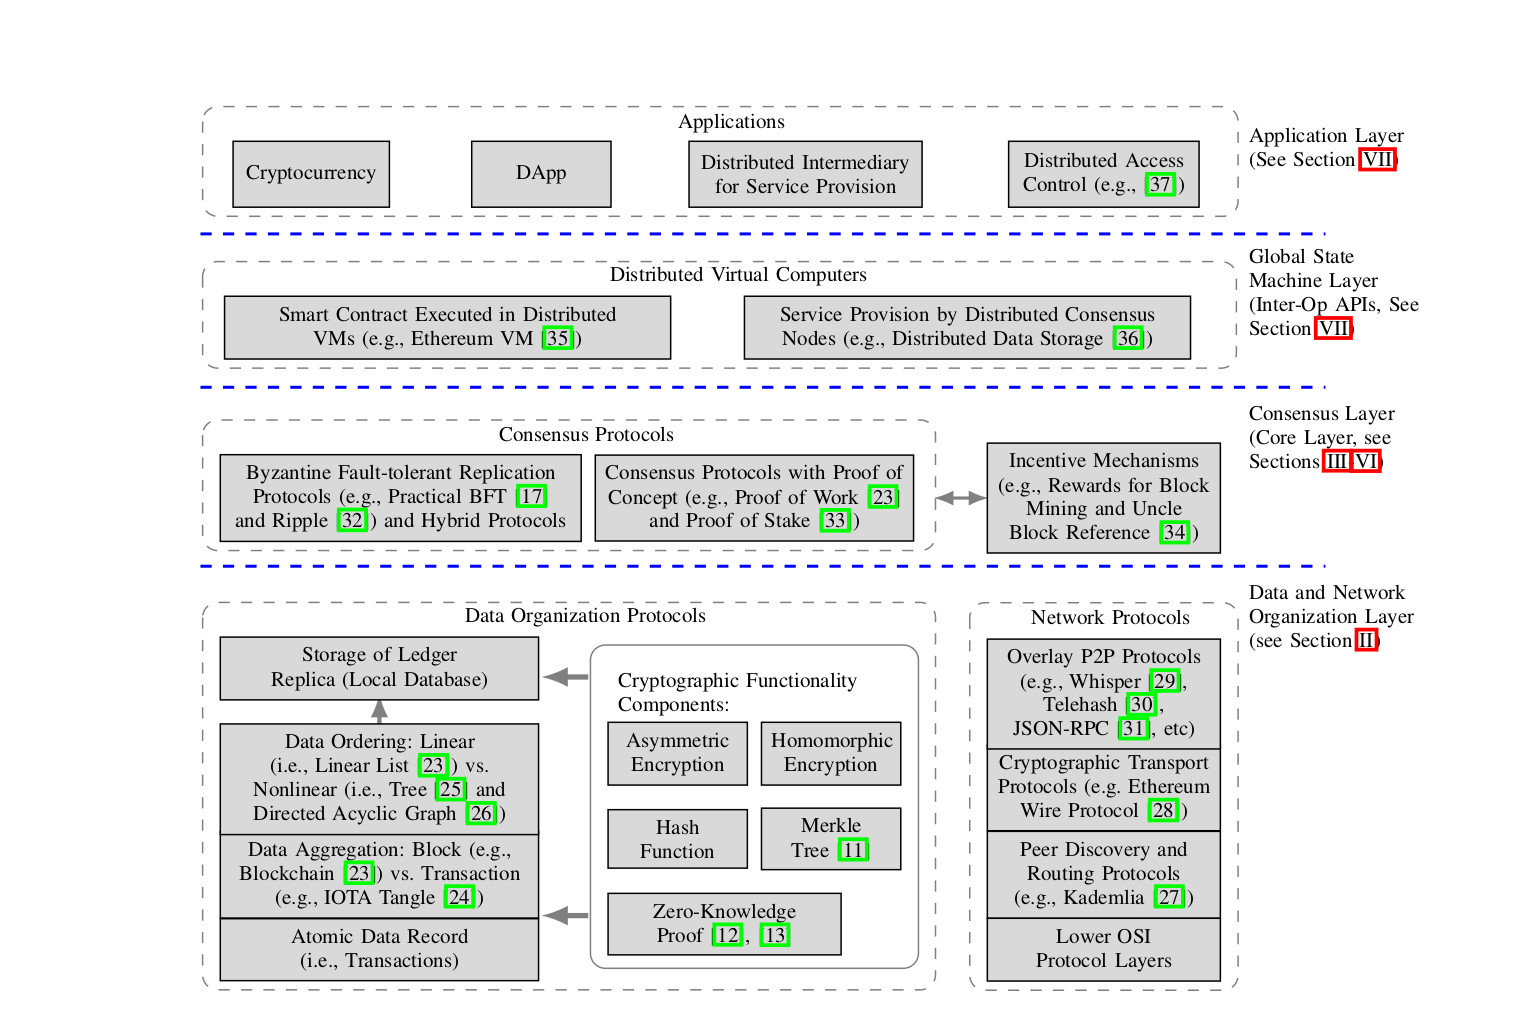
\includegraphics[width=1.95\textwidth]{images/chap02_BC_Tec_Stack.jpg}
 		\end{minipage}
 		\caption[Blochchainktechnology stack]{Blockchain technology stack}
 		
 	\end{figure}
 	
 \end{center}

\subsection{RDF graph}
\subsection{Graphchain Definition} Graphchain is blockchain mechanisim on the top of the RDF graph abtratc data type. An absttract RDF graph is the set of values and operations permitted on these value. This behaviour allows us to create be on the top of abstratc RDF graph data type. 
that gragraphsph hcian is:
\textit{linked chain of RDF graph is ordered linearly by functional relation referring to pervious graph in the chain.. THe first graph called genesis unit. }
\textit{the linked chain of RDF graph that used the blockchain mechanism such as hashing, linking of graphs, acheiving consensus, signature and so on.On the stored graphs in the multiple distributed database of chain RDF graph. The main benifit of this approach is the user can work with the chain of graphs with fully developed methods such : SPARQL for querying, linked data for access nodes on the graph and reasoning by the use of ontology and son on.[pp1171] }

\subsection{Graphchain Arciteture}

A single block contains some elements: \\
- web interface for communicating with the client via HTTP
- Web socket for communicating with other blocks.
- Module for handling calculation.
- Service to connect all this part together.
A client connects to block via HTTP to create new block and retrieve information from it. 
Clients connects to triple store via SPARQL HTTP allows to read data from it using SPARQL.
Nodes rae connected to each other using web socket protocol. In order to creating block, client, a HTTP request form client is needed that requests contains a RDF graph serialized in the turtle format.\\
There are some application to receive such format request then calculate hash and create new block.  
New block contains the blockchain header and content as a triple. new block arrange the triple in two sets: One triple of header store in graph ledger. Another one is triple of contents store as name graph. At the end, the modification publish to other nodes.[p1171]

\subsection{RDF Graf }
TODo

\subsection{Knowledge Graph}
One of the cornerstones of the Semantic Web is the ability to represent data
semantically { such that the meaning of a piece of data can be read, by human
	or machine, from the data itself and not from its position in a structure such as a
	relational table. The most commonly used standard is the Resource Description
	Framework (RDF) [26], in which data are represented as triples { semantically, predicate objec subject predicate ob-
				ject" sentences { where graphs serve to group triples. In both cases, subject and
					predicate (and graph, where present) are URIs, and objects may be either URIs
					or (optionally typed) literal values, e.g., numbers or strings. RDF has a number
					of concrete representation formats such as RDF/XML [6], Turtle [7], NTriples
					[5] and NQuads [10], JSON-LD [18], and so on, but each implement the same
					semantic model.
					Querying of Linked Data is designed around the idea that data from multiple
					sources can be linked easily no matter where it comes from, and without the need
					for coordination among data publishers beyond the use of common vocabularies
					and ontologies for common concepts. This model allows simple data integration
					and on-the-
y construction of relevant knowledge graphs from multiple sources
					by querying.
					The dominant standard for querying Linked Data is SPARQL [25]. A data
					source publishes a SPARQL endpoint, an HTTP-accessible interface which responds to queries in the SPARQL language, a query language which is somewhat
					similar to SQL [13], with SELECT, DELETE and INSERT operations (among
					others), and a query pattern syntax adapted to the RDF data model. It sup-
					ports sophisticated ltering and aggregation, and, crucially, via the SERVICE
					keyword, the ability to pass subqueries to other SPARQL endpoints to achieve
					federated querying { that is, querying of multiple data sources at once.
						The downside of SPARQL is its comparative weight on the server side, and
						its complexity. Many of the advanced ltering and aggregation features can be
						computationally expensive for the endpoint server executing them, and the im-
						plementation of SERVICE-based federated querying requires all communication
						between other data sources to be carried out by the initially targeted endpoint.
						To address these issues, the Linked Data Fragments (LDF) approach to
						querying has recently been proposed [1]. A data source for an LDF query may
						be a SPARQL endpoint, but can be any source which provides valid RDF. Cur-
						rently the only query patterns supported are Triple Pattern Fragments (TPF),
						although there is scope for extension. The basic query structure it handles is the
						Triple Pattern, which is an RDF triple { subject predicate object { but where
								one or more terms are replaced by variables in the form of alphanumeric strings
								beginning with a question mark. So where [53]